
\begin{abstract}
%When does multi-task learning provide positive (or negative) information transfer, compared to single-task learning?
	Multi-task learning is a powerful approach to solve complex tasks in many applications such as image and text classification.
	Yet, there is little rigorous understanding of when multi-task learning performs well, even compared to single-task learning.
	In this work, we study this question formally by considering three components including \textit{task similarity}, \textit{sample size} and \textit{covariate shift} in the setting of high-dimensional linear regression.
% the performance of predicting a particular task given multiple tasks.
%a multi-task learning architecture that uses a shared layer for all tasks and a separate output layer for each task.
	First, we show that whether multi-task learning performs better than single-task learning is determined by the bias-variance tradeoff of multi-task estimators.
	We analyze the bias-variance tradeoff by developing technical tools using random matrix theory.
	%we show that the type of transfer is determined by the bias-variance tradeoff of multi-task learning estimators.
	%We develop a technical tool to analyze the.
%	We develop a technical tool on the inverse of the sum of two random matrices that naturally arises from the analysis.
	Second, we apply our tools to show that the performance of multi-task learning is negatively affected as a result of: (a) decreased task similarity;
	(b) increased source sample size; (c) covariate shift under increased source sample size.
	Finally, we validate the three components of our theory on image and text classification tasks.
	Inspired by our theory, we propose an incremental training scheduler for improving the efficiency of multi-task training for predicting a particular task.
%	We validate our theory and our proposed method .
\end{abstract}

\section{Introduction}

%Multi-task learning is an inductive learning mechanism to improve generalization performance using related task data.
%Many state-of-the-art results in computer vision and natural language processing are obtained using multi-task learning.
Multi-task learning represents a powerful paradigm to solve complex tasks in computer vision \cite{chexnet17,ZSSGM18}, natural language processing \cite{GLUE,superglue} and many other areas \cite{ZY17}.
%In multi-task learning, having related task data is fundamental to its performance.
%Multi-task learning is particularly powerful when there is limited labeled data for a task to be solved, meanwhile more labeled data from different but related tasks is available.
%By combining multiple information sources, it is possible to share all the information in the same model.
In many settings, multiple information sources are available to help to solve a particular task.
%For example, many applications in , and many other areas have been achieved by learning from multiple tasks together.
The performance of multi-task learning depends on the relationship between the information sources and the task \cite{C97}.
When the information sources are heterogeneous, negative transfer--where multi-task learning (MTL)  performs worse than single-task learning (STL)--has often been observed \cite{PY09,AP16,BS17}.
While many empirical approaches are proposed to mitigate negative transfer \cite{ZY17}, a precise understanding of when negative transfer occurs remains elusive in the literature \cite{R17}.
%This phenomenon, known as \textit{negative transfer}, is fundamental to the understanding of multi-task learning.
In this work, we show that negative transfer is determined by the bias-variance tradeoff of multi-task learning estimators for the high-dimensional linear regression setting. % for learning from multiple linear regression tasks.
Moreover, we develop new tools to analyze the tradeoff and explain negative transfer precisely.
%Inspired by the theory, we propose an incremental training schedule to improve multi-task training.
%We consider a setting where the target task has limited labeled data and show
%On the other hand, unless the structures across task data are well-understood, applying multi-task learning on several different datasets often result in suboptimal models (or negative transfer in more technical terms).

Understanding negative transfer requires developing tight generalization bounds for both multi-task learning and single-task learning.
In classical Rademacher or VC based theory of multi-task learning \cite{B00,AZ05,M06}, the generalization bounds are usually presented so that the error reduces as the data sizes of all tasks increase.
For example, the sample sizes of all tasks are often assumed to be equal \cite{B00,LPTV09,LPVT11,MPR16}.
On the other hand, uneven sample sizes (or dominating tasks) have been empirically observed to cause negative transfer \cite{YKGLHF20}.
%The benefit of learning multi-task representations has also been studied for certain half-spaces \cite{} and sparse regression \cite{}.
When all tasks are sufficiently similar, adding more labeled data improves the generalization performance for predicting a particular task \cite{WZR20}.
To motivate our study, Figure \ref{fig_model_shift_phasetrans} shows three examples for two linear regression tasks solved using a shared linear layer for both tasks and an output layer for each task.
We observe that negative transfer occurs as (a) \textit{task similarity}: tasks become more different; (b) \textit{data size}: source/target data size increases.
%\textbf{Task similarity:}
%\textbf{Data sizes:}
%\textbf{Covariate shift:}
Furthermore, MTL performance is negatively affected when (c) \textit{covariate shift}: the covariance matrices of the two tasks become more different.
The observations highlight the need to develop generalization bounds that scale tightly with properties of multiple tasks data.

%\textbf{Setup and Main Results.}
Our main contribution is to develop technical tools to explain the above phenomena.
We focus on predicting a particular task given multiple high-dimensional linear regression tasks \cite{HMRT19,BLLT20}.
\squishlist
	\item \textbf{Task similarity:} We assume that each task follows a linear model with parameters $\beta_i\in\real^p$, for $1\le i\le t$.
	Hence, task similarity can be measured by the distance between the model parameters.
	\item \textbf{Sample size:} Let $n_i = \rho_i \cdot p$ denote the sample size of task $i$, for a fixed value $\rho_i > 1$ that does not grow with $p$, for any $1\le i\le t$.
	Hence, for a source task $s$ and a target task $t$, their data ratio is measured by $n_s / n_t = \rho_s / \rho_t$.
	Importantly, we assume that for the $t$-th (target) task, $\rho_t$ is a small constant (say 2), to capture the need for adding more labeled data.
	\item \textbf{Covariate shift:} We assume that for every task $1\le i\le t$, its features are random vectors with covariance matrix $\Sigma_i\in\real^{p\times p}$.
	%$x = \Sigma_i^{1/2}z$, where $z\in\real^p$ consists of i.i.d. entries with mean zero and unit variance, and is a positive semidefinite matrix.
	Given two tasks $i$ and $j$, we measure covariate shift by $\Sigma_i^{1/2}\Sigma_j^{-1/2}$.
\squishend
% that only contains limited amount of labeled data.
%Following Hastie et al.  and Bartlett et al. \cite{},

%Let $n_i = \rho_i \cdot p$ denote the data size and $X_i\in\real^{n_i\times p}$ denote the features of task $i$.
%The labels of task $i$ are given by $Y_i = X_i\beta_i + \varepsilon_i$, where $\beta_i\in\real^p$ denotes task $i$'s ground truth parameters and $\varepsilon_i$ denotes i.i.d. random noise with mean zero and variance $\sigma^2$.
We focus on the hard parameter sharing architecture with a linear shared layer for all tasks and a separate prediction head for each task \cite{R17,WZR20,MTDNN19}.
%This corresponds to minimizing $ \sum_{i=1}^t \norm{X_i B W_i - Y_i}^2$.
Let $\hat{\beta}_t^{\MTL}$ denote the optimal multi-task estimator for the target task, which is defined precisely in Section \ref{sec_setup}.
We revisit the bias-variance tradeoff of $\hat{\beta}_t^{\MTL}$.
Interestingly, we observe that the variance of the multi-task estimator is always smaller than the variance of the single-task estimator, because of an increased sample size.
The bias of the multi-task estimator results in a negative effect caused by the difference between $\beta_t$ and the rest of $\set{\beta_i}_{i=1}^{t-1}$.
Hence, the bias-variance tradeoff determines whether we observe positive or negative transfer.
For the setting of two tasks, we show how the variance of the multi-task estimator  scales with sample size and covariate shift in the following result.
%\textit{Our first contribution} is to develop a concentration bound that arises naturally from the bias-variance tradeoff of $\hat{\beta}_t^{\MTL}$ for two tasks.
%Let $\hat{\beta}_t^{\STL}$ denote the single-task estimator.
%Without loss of generality, let the $t$-th task denote the target task.
%Importantly, the target task's data size is a fixed constant times $p$ in the high-dimensional setting.
%Hence adding more labeled data can help improve its test performance.
%$B\in\real^{p\times r}$
%$\set{W_i \in \real^{r}}_{i=1}^t$

\begin{figure}[!t]
	\begin{subfigure}[b]{0.32\textwidth}
		\centering
		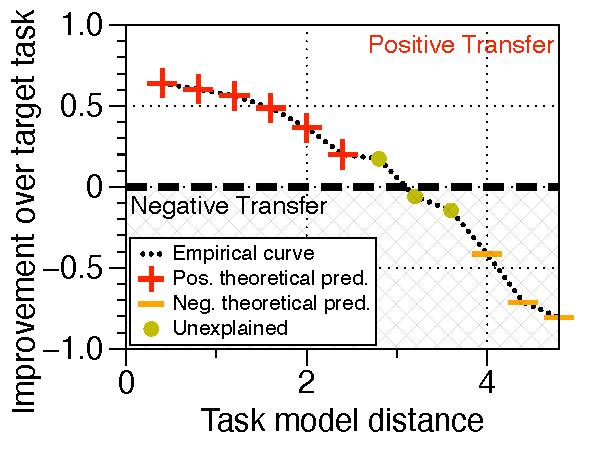
\includegraphics[width=0.98\textwidth]{figures/model_shift_phase_transition.pdf}
		\vspace{-0.075in}
		\caption{Task similarity}
		\label{fig_model_shift}
	\end{subfigure}\hfill
	\begin{subfigure}[b]{0.32\textwidth}
		\centering
		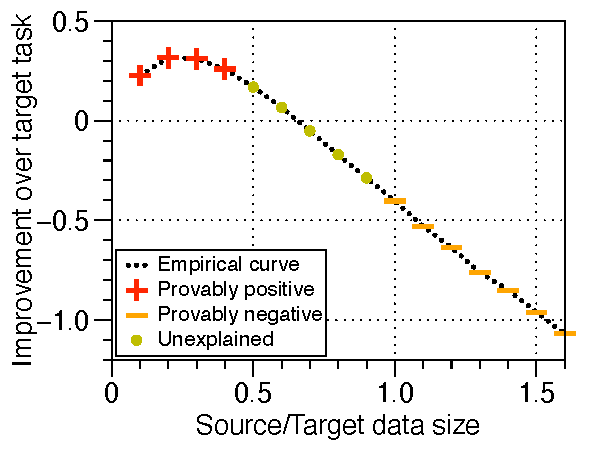
\includegraphics[width=0.98\textwidth]{figures/datapoints_phase_transition.pdf}
		\vspace{-0.075in}
		\caption{Sample size}
		\label{fig_size}
	\end{subfigure}\hfill
	\begin{subfigure}[b]{0.32\textwidth}
		\centering
		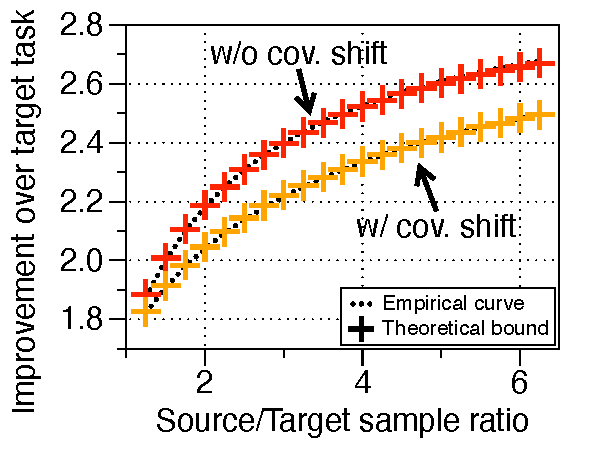
\includegraphics[width=0.98\textwidth]{figures/complementary.pdf}
		\vspace{-0.075in}
		\caption{Covariate shift}
		\label{fig_covariate}
	\end{subfigure}
	\caption{%Three takeaways of our theory in Section \ref{sec_insight}.
	We observe that MTL performance
	(a) undergoes transition from positive to negative transfer as \textit{task model distance} increases (Prop.\;\ref{prop_dist_transition});
	(b) undergoes transition from positive to negative transfer as source/target \text{sample size} increases (Prop.\;\ref{prop_data_size});
	(c) gets worse as \textit{covariate shift} gets more severe (larger $\lambda$) and source/target \textit{sample size} increases (Prop.\;\ref{prop_covariate}).
	The $y$-axis measures the loss of STL minus MTL.}
	\label{fig_model_shift_phasetrans}
	\vspace{-0.1in}
\end{figure}


%Concretely, we show a tight bound on the trace of $(X_1^{\top}X_1 + X_2^{\top}X_2)^{-1}$, which
Theorem \ref{lem_cov_shift_informal} allows us to analyze the bias-variance tradeoff of the multi-task estimator for two settings:
(i) two tasks with arbitrary covariate shift; (ii) many tasks with no covariate shift.

%We shall assume that each task data follows a linear model, i.e. $y_i = X_i \beta_i + \varepsilon_i$, $1\le i\le k$.
%Here $\beta_i\in\real^p$ is the model parameter for the $i$-th task.
%Each row of $X_i\in\real^{n_i\times p}$ is assumed to be drawn i.i.d. from a fixed
%distribution with covariance matrix $\Sigma_i$.

%We extend our result to the transfer learning
%in the setting of high-dimensional linear regression.
%by pooling source task representations into the shared body of the hard parameter sharing architecture, following
%setting of Taskonomy by Zamir et al. \cite{ZSSGM18}.
%We prove that the bias of the transfer learning estimator is given by the projection of $\beta_t$ to the orthogonal subspace spanned by $\set{\beta_i}_{i=1}^{t-1}$.
%These results are described more precisely in Section \ref{sec_main}.

Next, we use our newly developed tool to explain negative transfer in multi-task learning precisely.
In Section \ref{sec_insight}, we explain the three phenomena in Figure \ref{fig_model_shift_phasetrans} for a simplified isotropic setting of two tasks.
It is crucial that the concentration result in Theorem \ref{lem_cov_shift_informal} is sufficiently precise so that we can explain the transition phenomena in Figure \ref{fig_model_shift} and \ref{fig_size}.
The unexplained observations are caused by an error term that arises from the bias of $\hat{\beta}_t^{\MTL}$ -- we discuss these in Section \ref{sec_insight} more precisely.
Theorem \ref{lem_cov_shift_informal} allows us to compare MTL performance under different covariate shifts.
When task models are the same and the covariate shift matrix belongs to a certain bounded set, we show that having no covariate shift yields the optimal MTL performance.
%In Section \ref{sec_insight}, we consider three components including task similarity, data size and covariate shift for a simplified isotropic setting of two tasks.
%We measure task similarity by how small is the distance between $\beta_1$ and $\beta_2$.
%Using our tool, we explain a transition from positive to negative transfer as task similarity decreases.
%		Furthermore, we show that negative transfer is more likely to occur when the source task labels are particularly noisy.
%		In Section \ref{sec_validate}, we validate the observation on text and image classification tasks.
%	In , we provide the trade-off between $\norm{\beta_1 - \beta_2}^2$ and a certain function $\Phi(\rho_1, \rho_2)$ to determine the type of transfer.
%We show that increasing the data size of the source task does not always improve performance for the target task in multi-task learning.
Finally, we analyze the benefit of MTL for reducing the amount of labeled data needed to achieve comparable performance to STL, which is a key empirical finding of Taskonomy.
%We show that covariate shift, measured by $\Sigma_1^{1/2}\Sigma_2^{-1/2}$, is another cause for suboptimal performance for $\hat{\beta}_t^{\MTL}$.
%		We show that as $n_1 / n_2$ becomes large, having no covariate shift between the source and target tasks yields the optimal performance for the target task.
%		On the other hand, when $n_1 / n_2$ is small, there are counter examples where having the same covariance matrix is not necessarily the optimal choice.

\textit{Our last contribution} is to connect our theory to practical problems of interest.
(i) We validate the three components of our theory in Section \ref{sec_insight} and measure the data efficiency of multi-task learning on the sentiment analysis dataset.
(ii) We provide a single-task based metric to predict positive or negative transfer in multi-task learning.
While it is not well understood when multi-task learning provides positive transfer, we show that the STL results can help indicate and understand MTL results on ChestX-ray14 \cite{chexnet17} and sentiment analysis datasets \cite{LZWDA18}.
(iii) We design an incremental training schedule to improve the efficiency of multi-task training for predicting a particular task.
We show that our training schedule reduces the computational cost by $55\%$ compared to baseline multi-task training on the sentiment analysis dataset, while keeping the accuracy the same.

